\begin{problem}{Joined Vessels}{standard input}{standard output}{3 seconds}{512 megabytes}

John is doing physics practice at school. Today he is studying the law of communicating vessels. This law states that if we have a set of communicating containers with a homogeneous liquid, when the liquid settles, it balances out to the same level in all of the containers regardless of their shape and volume.

In the lab, John has a set of $n$ cylindrical vessels with a base area of one square decimeter and a height that we consider to be infinite. The vessels are numbered from $1$ to $n$, and vessels $i$ and $i+1$ are communicating via a very thin bridge at a height of $h_i$ decimeters. All these heights are pairwise distinct.

The practice work contains $t$ independent experiments. In each experiment, all vessels are initially empty. In the $i$-th experiment, water is slowly put into vessel $a_i$, and the experiment finishes when any amount of water appears in vessel $b_i$. 
The result of the experiment is the total volume of water put into vessel $a_i$, measured in liters (or, equivalently, cubic decimeters).

Note that the law of communicating vessels can only be applied to vessels $i$ and $i+1$ when the water level is at least $h_i$ in both of them. Until then, if the water level reaches $h_i$ in just one of them, it stays constant and any excess water coming into this vessel flows through the bridge into the other one.

Help John check his results!

\InputFile
The first line of the input contains an integer $n$~--- the number of vessels ($2 \le n \le 2 \cdot 10^5$). 

The second line contains $n - 1$ integers $h_1, h_2, \dots, h_{n-1}$~--- the heights of communication bridges between consecutive vessels, in decimeters ($1 \le h_i \le 10^9$). These heights are pairwise distinct.

The third line contains an integer $t$~--- the number of experiments ($1 \le t \le 2 \cdot 10^5$).

Each of the following $t$ lines contains two integers $a_i$ and $b_i$~--- the numbers of the starting vessel and the target vessel in the $i$-th experiment ($1 \le a_i \le n$; $1 \le b_i \le n$; $a_i \neq b_i$).

\OutputFile
For each experiment, in the order of input, output a single integer~--- the required volume of water, in liters. 

\Example

\exmpthreewidinf=0.22\thelinewidth
\exmpthreewidouf=0.22\thelinewidth
\exmpthreewidnote=0.46\thelinewidth
\def\kwExampleNotes{Illustration}



\begin{examplethree}
\exmp{6
1 4 2 3 5
4
1 6
6 1
2 5
5 2
}{25
18
14
12
}{
\vspace{-1mm}
\center
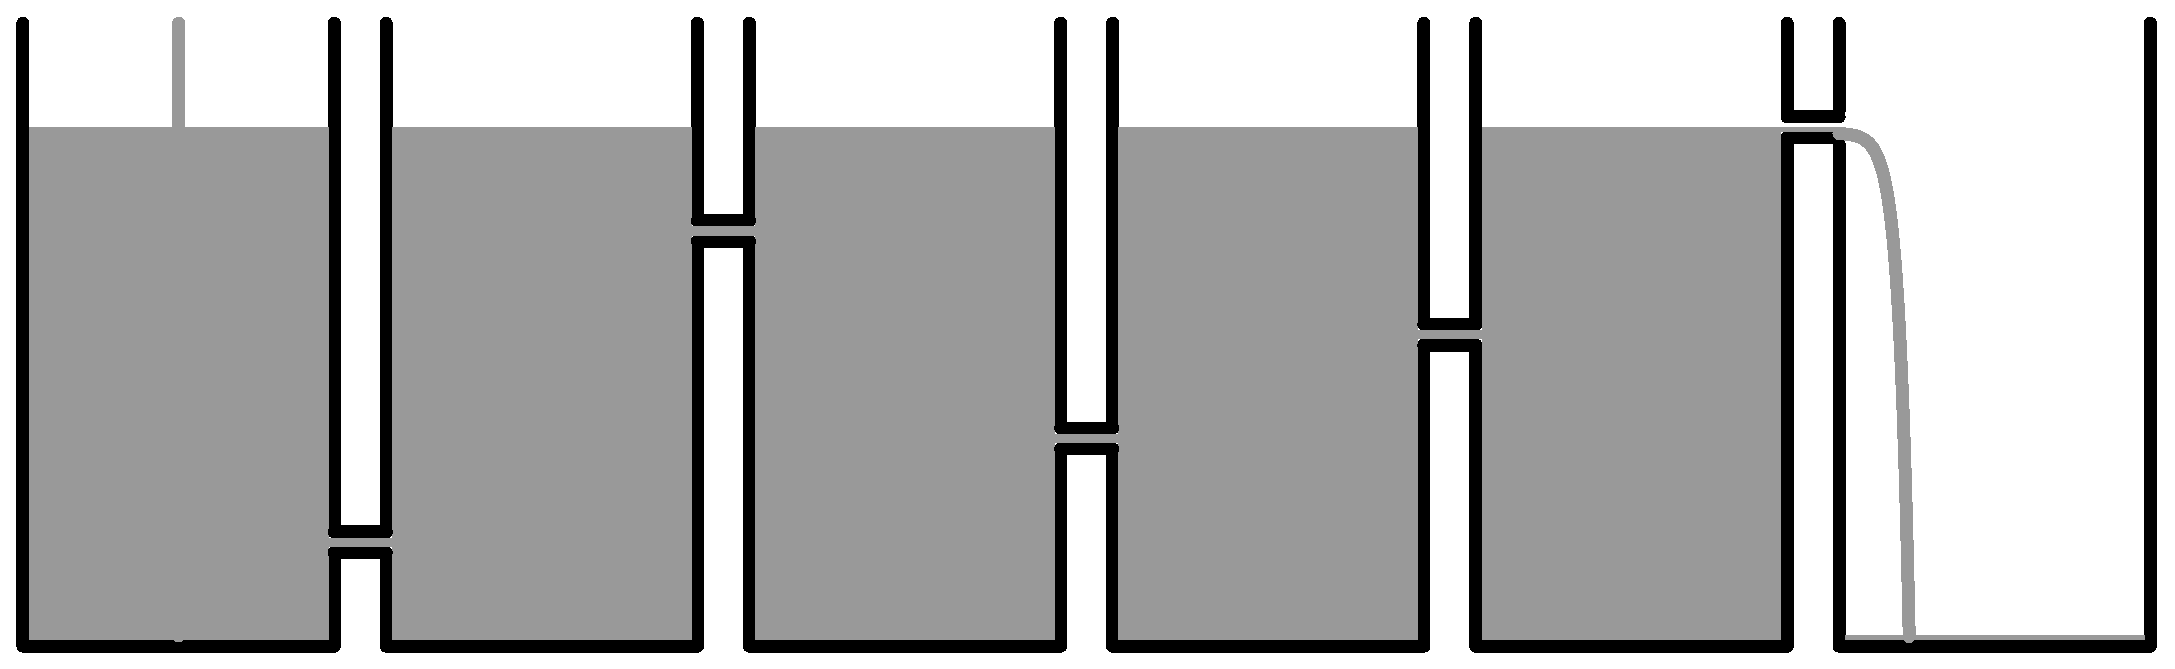
\includegraphics[scale=0.15]{joined-1.eps}
\vspace{2mm}
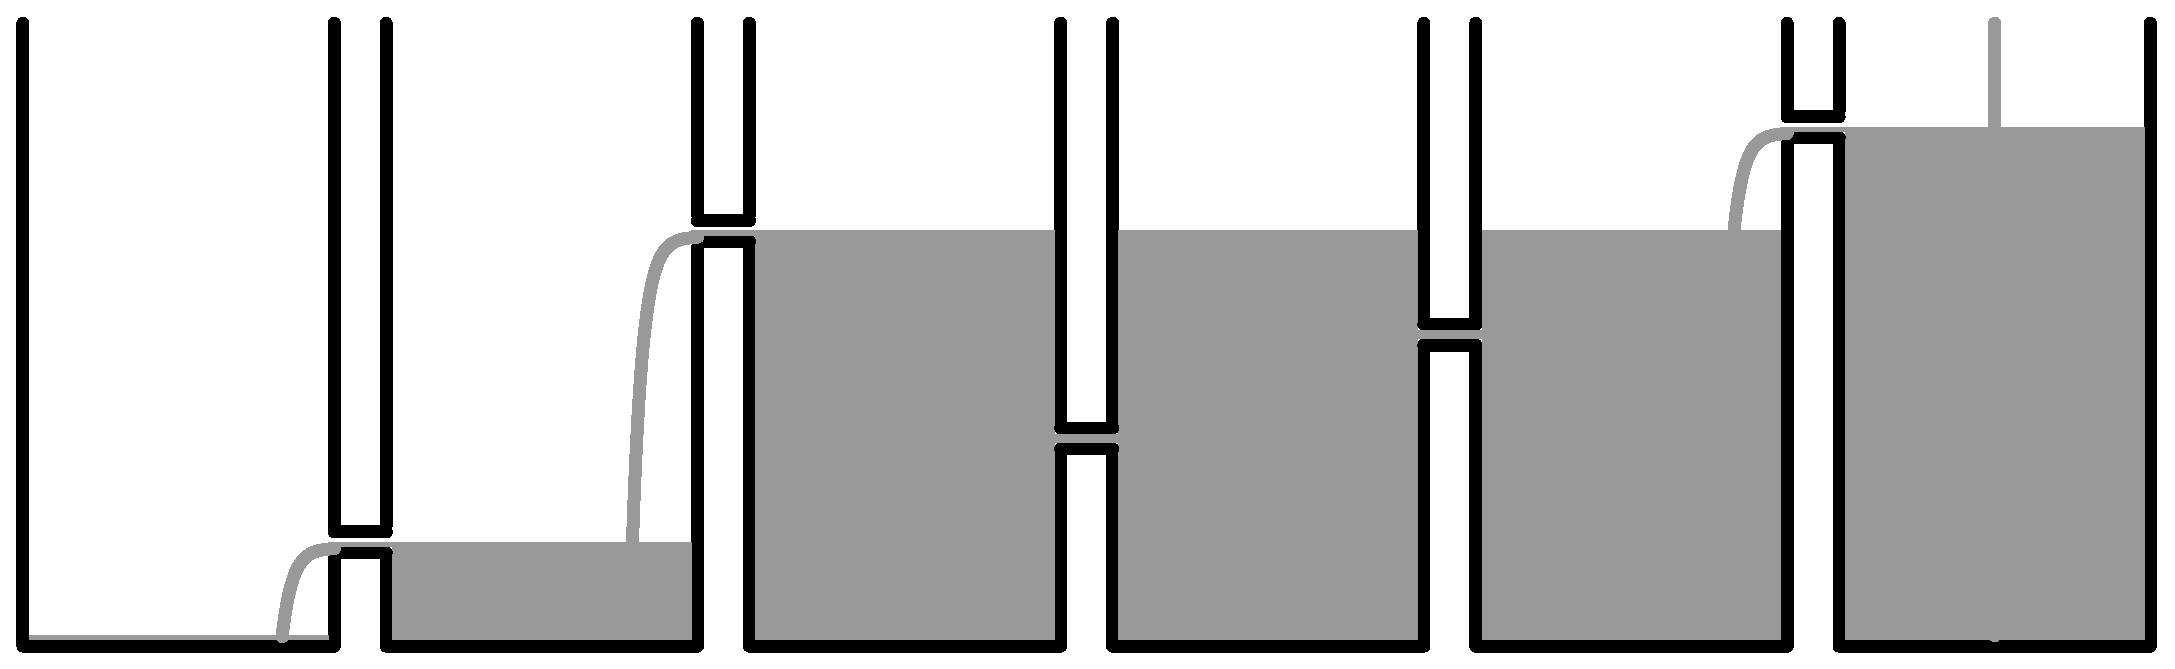
\includegraphics[scale=0.15]{joined-2.eps}
\vspace{2mm}
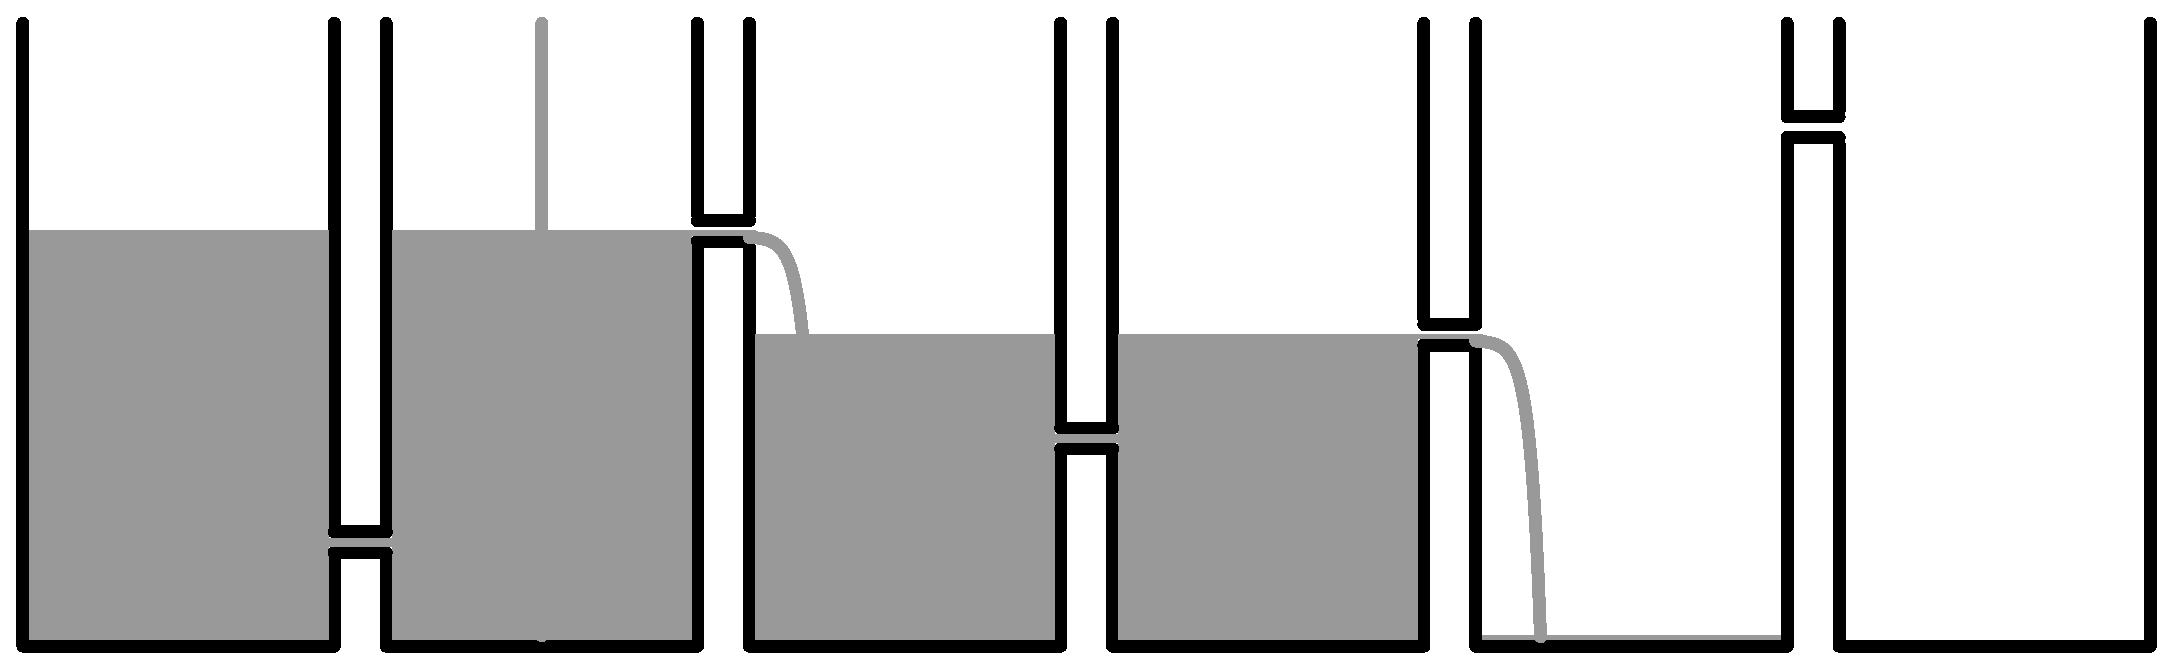
\includegraphics[scale=0.15]{joined-3.eps}
\vspace{2mm}
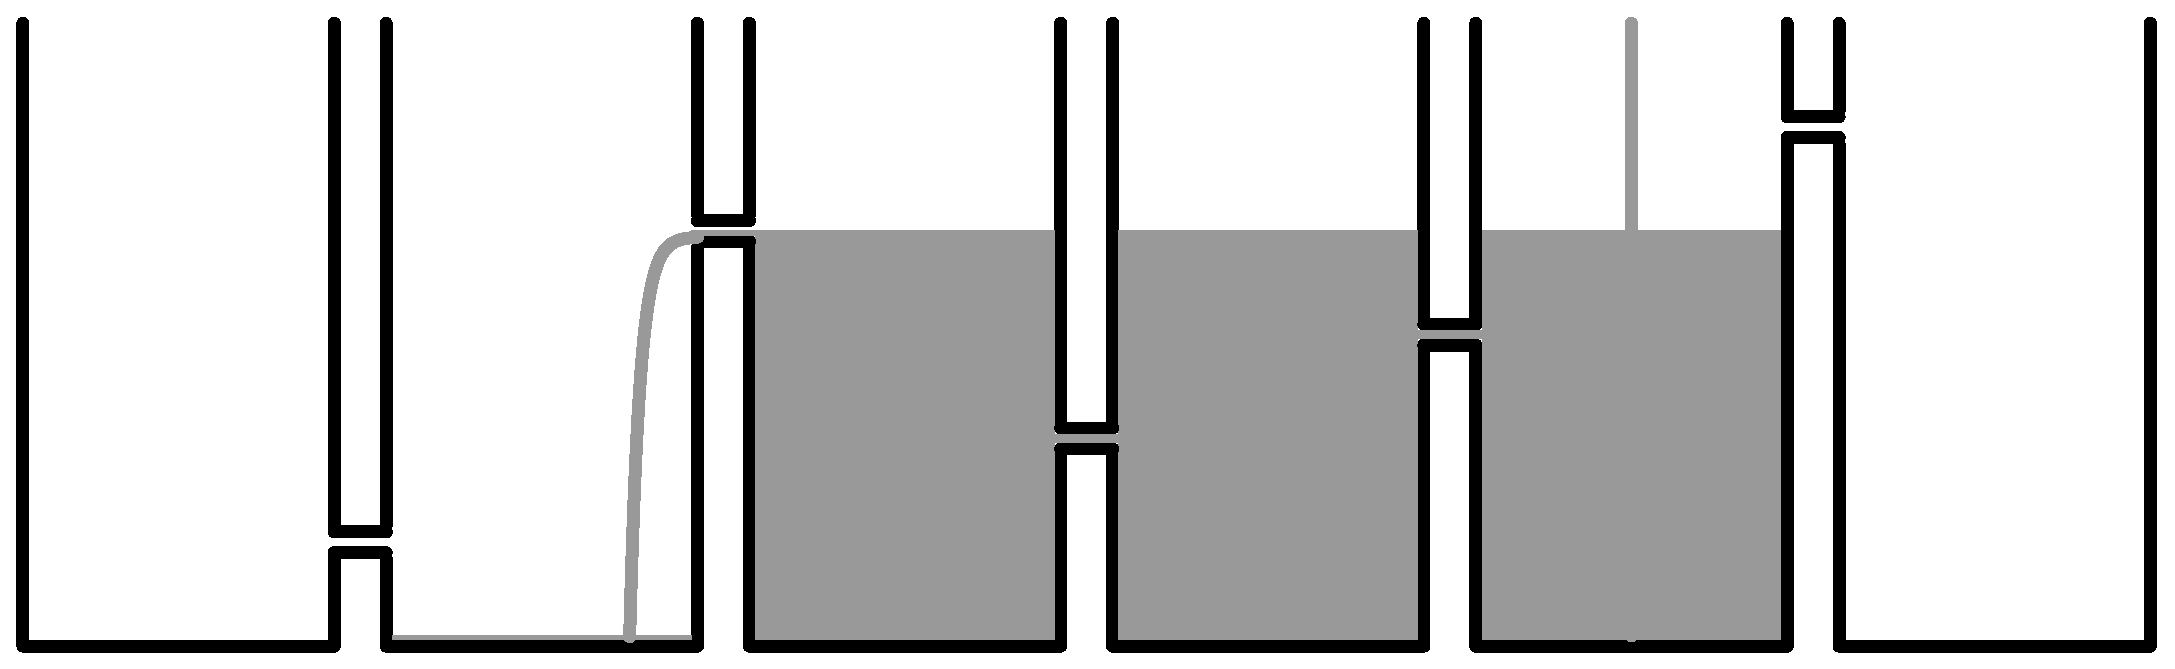
\includegraphics[scale=0.15]{joined-4.eps}
\vspace{2mm}
}%
\end{examplethree}

\end{problem}

